\documentclass[11pt,a4paper]{article}
\usepackage[utf8]{inputenc}
\usepackage[T1]{fontenc}
\usepackage[provide=*]{babel}
\babelprovide[main,import]{french}
\IfFileExists{lmodern.sty}{\usepackage{lmodern}}{}
\usepackage[a4paper,margin=2.5cm]{geometry}
\usepackage{setspace}
\onehalfspacing
\usepackage{amsmath}
\usepackage{array}
\usepackage{microtype}
\usepackage{graphicx}
% Les images (logos AMU/AMSE, signature) vivent dans Memoire/logos/.
\graphicspath{{../logos/}{logos/}{./}}
\usepackage{xcolor}
\usepackage{fancyhdr}
\IfFileExists{xurl.sty}{\usepackage{xurl}}{}
\usepackage[hidelinks]{hyperref}
\usepackage{ragged2e}\hypersetup{colorlinks=true, linkcolor=black, urlcolor=blue!50!black, citecolor=black}
\IfFileExists{float.sty}{\usepackage{float}}{}
\IfFileExists{booktabs.sty}{\usepackage{booktabs}}{}
\IfFileExists{tabularx.sty}{\usepackage{tabularx}}{}
\IfFileExists{tikz.sty}{\usepackage{tikz}\usetikzlibrary{arrows.meta,positioning}}{}
\definecolor{myblue}{RGB}{35,55,120}
\definecolor{mygreen}{RGB}{42,120,80}
\definecolor{myred}{RGB}{145,55,55}
\definecolor{mygray}{RGB}{85,85,85}
\IfFileExists{titlesec.sty}{%
  \usepackage{titlesec}%
  \titleformat{\section}{\large\bfseries\color{myblue}}{\thesection.}{0.5em}{}%
  \titleformat{\subsection}{\normalsize\bfseries\color{myblue!85}}{\thesubsection.}{0.5em}{}%
  \titlespacing*{\section}{0pt}{1.2\baselineskip}{0.6\baselineskip}%
  \titlespacing*{\subsection}{0pt}{1.0\baselineskip}{0.45\baselineskip}%
  \titlespacing*{\subsubsection}{0pt}{0.8\baselineskip}{0.35\baselineskip}%
}{}
\pagestyle{fancy}\fancyhf{}
\fancyhead[L]{\footnotesize Rapport de stage, M2 Econometrics \& Statistics}
\fancyhead[R]{\footnotesize J.D'OLIVEIRA}
\fancyfoot[C]{\thepage}
\setlength{\headheight}{14pt}

% Repli si une image n'est pas encore fournie (logos AMU/AMSE, signature).
% Des que le .png est depose dans ce dossier, il est utilise automatiquement.
\newcommand{\imgOrPlaceholder}[3]{%
  \IfFileExists{../logos/#2}{\includegraphics[#1]{../logos/#2}}{%
   \IfFileExists{logos/#2}{\includegraphics[#1]{logos/#2}}{%
    \IfFileExists{#2}{\includegraphics[#1]{#2}}{%
     \fbox{\parbox[c][1.4cm][c]{4.2cm}{\centering\scriptsize\color{red}\textbf{#3}\\[1mm]fichier \texttt{#2} absent}}}}}%
}

\newcommand{\rapportdate}{22 août 2026}

\begin{document}
\hypersetup{pageanchor=false}
\pagenumbering{gobble}

% ============================ PAGE DE TITRE ============================
\begin{titlepage}
\centering
\vspace*{1.5cm}
{\scriptsize AIX-MARSEILLE UNIVERSITÉ, AIX-MARSEILLE SCHOOL OF ECONOMICS\par}
{\scriptsize Master Econometrics \& Statistics, M2 Econometrics, Data Science (EDS)\par}
\vspace{2cm}
{\color{myblue}\rule{\textwidth}{1.2pt}}\\[0.6cm]
{\LARGE\bfseries Constitution d'une banque de données de référence pour la validation de modèles prédictifs spatio-temporels\par}
\vspace{0.4cm}
{\large\itshape D'un système de métadonnées enrichies à un banc d'essai exécutable\par}
{\color{myblue}\rule{\textwidth}{1.2pt}}\\[1.2cm]

{\large\textbf{Johnny D'OLIVEIRA}\par}
\vspace{1.5cm}
\begin{tabular}{>{\bfseries}p{4.9cm}p{8.9cm}}
Organisme d'accueil & INRAE, Centre d'Avignon, unité Écodéveloppement \\[0.2cm]
Encadrant professionnel & Ghislain Geniaux, chargé de recherche à l'INRAE \\[0.2cm]
Encadrement académique & Badih GHATTAS et Pierre Michel, responsables du parcours EDS, AMSE \\[0.2cm]
Période & Avril à septembre 2026 \\
\end{tabular}
\vfill
{\footnotesize Rapport de stage de fin d'études, \rapportdate\par}
\end{titlepage}

% ============================ PAGE NON-PLAGIAT ============================
\thispagestyle{empty}
% Logos
\noindent
\begin{minipage}{0.45\textwidth}
    \imgOrPlaceholder{height=1.5cm}{logo_amu.png}{LOGO AMU}
\end{minipage}
\hfill
\begin{minipage}{0.45\textwidth}
    \raggedleft
    \imgOrPlaceholder{height=1.5cm}{logo_amse.png}{LOGO AMSE}
\end{minipage}

\vspace{3.5cm}

\begin{center}
    \textbf{\Large ENGAGEMENT DE NON-PLAGIAT}
\end{center}

\vspace{3cm}

\noindent
Je soussigné, \textit{Johnny D'OLIVEIRA},
déclare être pleinement conscient que le plagiat, consistant à copier des documents ou une partie d'un document publié sous quelque forme que ce soit et sur quelque support que ce soit, y compris les publications en ligne, constitue une violation du droit d'auteur et des droits voisins, ainsi qu'une fraude pure et simple.

\vspace{0.5cm}

\noindent
En conséquence, je m'engage par la présente à citer toutes les sources et tous les auteurs auxquels j'ai eu recours pour rédiger mon rapport de stage et ses annexes.

\vspace{2cm}

\noindent
\begin{minipage}[t]{0.45\textwidth}
Date : \rapportdate
\end{minipage}
\hfill
\begin{minipage}[t]{0.45\textwidth}
\raggedleft
\begin{minipage}[t]{3.5cm}
\centering
Signature:

\vspace{0.2cm}

\imgOrPlaceholder{width=2.5cm}{signature.png}{SIGNATURE}\\[-0.1cm]
Johnny D'OLIVEIRA
\end{minipage}
\end{minipage}

\newpage

% ============================ TABLE DES MATIERES ============================
\thispagestyle{empty}
\tableofcontents
\newpage
\hypersetup{pageanchor=true}
\pagenumbering{arabic}

% ============================ INTRODUCTION ============================
\section{Introduction}

Ce rapport rend compte du stage de fin d'études réalisé au sein de l'unité Écodéveloppement de l'INRAE, au centre d'Avignon. Il présente la mission qui m'a été confiée et en propose une lecture analytique à partir des compétences acquises durant le Master. La problématique de départ est méthodologique. Il s'agit de déterminer comment valider de manière crédible des méthodes statistiques destinées aux données spatiales et spatio-temporelles lorsque les jeux de données de référence disponibles restent peu nombreux, dispersés et difficilement comparables.

La validation d'une méthode prédictive peut emprunter trois voies complémentaires. La première consiste à établir mathématiquement ses propriétés, notamment asymptotiques. Une telle démonstration n'est toutefois pas toujours accessible pour des estimateurs complexes. La deuxième repose sur des simulations de Monte-Carlo. Comme le processus générateur des données est connu, celles-ci permettent d'évaluer à la fois la qualité de l'inférence sur les paramètres et la capacité prédictive du modèle. Elles occupent ainsi une place importante dans l'évaluation des méthodes statistiques.

 Les simulations présentent néanmoins une limite importante. Elles ne peuvent couvrir qu'un nombre restreint de configurations, alors que les données spatiales et spatio-temporelles peuvent combiner des distributions non normales, des corrélations entre variables, des non-linéarités, des interactions ou encore des erreurs de mesure. Aucun plan de simulation ne peut reproduire toute cette diversité. Une troisième voie consiste donc à confronter les méthodes à des données réelles et variées. Elle permet d'observer leur comportement dans des situations qui n'ont pas été entièrement construites par l'expérimentateur.


Cette approche possède elle aussi ses limites. Sur des données réelles, les véritables paramètres du processus générateur sont inconnus. Il devient alors possible d'évaluer la capacité prédictive d'un modèle, mais beaucoup plus difficile de juger directement la qualité de l'inférence sur ses paramètres. Une banque de données réelles ne remplace donc pas les expériences de Monte-Carlo. Elle constitue une couche de validation complémentaire. Cette distinction est particulièrement importante pour les méthodes d'apprentissage automatique, puisqu'un modèle peut fournir de bonnes prédictions sans nécessairement permettre une interprétation correcte des effets des variables, notamment en présence d'endogénéité.


C'est dans cette troisième voie qu'apparaît une difficulté structurelle. De nombreux jeux de données réels existent, mais ils sont rarement disponibles sous une forme homogène. Leur documentation ne permet pas toujours de retrouver facilement la variable réponse, les covariables, la structure spatiale ou la spécification utilisée dans la publication d'origine. Ils sont également dispersés entre articles scientifiques, packages statistiques et entrepôts de données. Cette difficulté n'est pas propre aux méthodes spatiales. En apprentissage automatique, des initiatives telles que PMLB ont cherché à regrouper et standardiser des jeux de données afin de faciliter l'évaluation comparative des méthodes (Olson \textit{et al.}, 2017). Plus généralement, la littérature sur le benchmarking des méthodes computationnelles souligne l'importance de disposer de protocoles et de ressources partagés pour rendre les comparaisons plus transparentes et reproductibles (Weber \textit{et al.}, 2019 ; Thiyagalingam \textit{et al.}, 2022).


Les données spatiales ajoutent une difficulté supplémentaire. Les observations proches géographiquement peuvent être dépendantes, ce qui remet en cause certains protocoles classiques d'évaluation fondés sur l'indépendance entre les échantillons d'entraînement et de test. La constitution d'une banque de référence dans ce domaine suppose donc non seulement de rassembler des jeux de données, mais aussi de documenter suffisamment leur structure pour permettre l'utilisation de protocoles de validation adaptés.

L'objectif de mon stage est de contribuer à la construction d'une telle banque de données de référence. Celle-ci est conçue comme un banc d'essai structuré plutôt que comme une simple accumulation de jeux disponibles. Le travail comprend également le développement d'une infrastructure logicielle permettant de documenter, préparer et exploiter ces données dans des conditions comparables.

Le rapport est organisé en trois parties principales. La première présente le contexte du stage, l'organisme d'accueil et l'écosystème scientifique dans lequel s'inscrit la mission. La deuxième décrit le travail réalisé, depuis la constitution et la documentation de la banque jusqu'au développement de l'infrastructure permettant d'exécuter les benchmarks. Elle revient également sur les difficultés rencontrées et sur les solutions mises en place. La conclusion propose enfin un bilan du travail accompli, de ses limites et des apports du Master dans sa réalisation.
% ============================ CONTEXTE ============================
\section{Contexte}

Cette section présente l'environnement scientifique et institutionnel dans lequel s'est déroulé le stage. Elle revient d'abord sur l'organisme et l'unité d'accueil, puis sur l'écosystème de science ouverte mobilisé au cours de la mission. Elle permet enfin de situer les principaux éléments qui ont facilité le travail ainsi que les contraintes auxquelles il a fallu répondre.

\subsection{L'organisme d'accueil}

L'INRAE, Institut national de recherche pour l'agriculture, l'alimentation et l'environnement, est un établissement public de recherche français issu de la fusion, en 2020, de l'INRA et d'IRSTEA. Ses activités portent sur les enjeux liés à l'agriculture, à l'alimentation et à l'environnement. Sa production repose principalement sur la création et la diffusion de connaissances scientifiques, notamment sous la forme de publications, de logiciels et de jeux de données. Dans ce contexte, la valeur d'un travail de recherche tient moins à une logique marchande qu'à la robustesse, à la reproductibilité et à la capacité de réutilisation des résultats produits.

Le stage s'est déroulé au sein de l'unité Écodéveloppement, rattachée au centre INRAE Provence-Alpes-Côte d'Azur et au département ACT, « Sciences pour l'action, les transitions, les territoires ». Ce département étudie notamment les transformations des socio-écosystèmes et des systèmes agroalimentaires, avec l'objectif d'accompagner les transitions vers la durabilité et d'éclairer l'action publique.

Créée en 1983 autour du concept d'écodéveloppement, l'unité a progressivement élargi ses approches disciplinaires et ses objets de recherche. À partir des années 1990, elle a notamment accueilli des travaux en économie et en sociologie sur les politiques publiques agro-environnementales. L'analyse spatiale occupe également une place ancienne dans ses recherches. Dès les années 2000, certaines problématiques foncières ont été étudiées à l'aide de l'économétrie spatiale.

Aujourd'hui, les travaux de l'unité portent notamment sur la compréhension et l'accompagnement de l'écologisation des systèmes agroalimentaires, à différentes échelles allant des systèmes de production aux territoires. L'unité se caractérise par une forte interdisciplinarité. Elle réunit notamment des agronomes, des sociologues, des économistes, des géographes et des écologues, et mobilise aussi bien des méthodes qualitatives que des méthodes quantitatives telles que l'économétrie, la géomatique et l'analyse spatiale.

C'est dans ce cadre que s'inscrit une activité méthodologique consacrée au développement de méthodes statistiques pour les données spatiales et spatio-temporelles. Cette expertise se traduit notamment par le développement de packages R. Le package \texttt{mgwrsar}, par exemple, propose des méthodes permettant de traiter conjointement l'autocorrélation et l'hétérogénéité spatiales (Geniaux \& Martinetti, 2018). D'autres travaux portent sur des approches multi-échelles à fenêtres localement adaptatives (Geniaux, 2026) ainsi que sur des méthodes de boosting spatialisé. Le stage a été encadré par Ghislain Geniaux, chargé de recherche à l'INRAE et auteur de plusieurs de ces travaux.

Ces activités expliquent directement l'intérêt de la mission pour l'unité. Le développement d'un nouvel estimateur ne suffit pas à établir son comportement empirique. Il faut également pouvoir l'évaluer sur des configurations spatiales variées et le comparer à des méthodes existantes dans des conditions homogènes. La banque de données construite pendant le stage vise à fournir progressivement ce matériel commun d'évaluation.

\subsection{Un écosystème de recherche ouvert}

La mission dépasse le seul cadre de l'unité d'accueil. Elle repose largement sur l'écosystème de la science ouverte, aussi bien pour découvrir des jeux de données que pour documenter leur provenance.

Les données et leurs métadonnées peuvent provenir de plusieurs types de sources. Certaines sont publiées dans des entrepôts comme Zenodo ou Dryad, d'autres sont accessibles depuis des portails institutionnels tels que l'INSEE ou Eurostat. Des infrastructures comme OpenAlex, Crossref ou DataCite permettent par ailleurs d'identifier les publications, leurs Digital Object Identifier (DOI) et les ressources qui leur sont associées.

Ces services ne fournissent donc pas uniquement des fichiers. Ils donnent également accès à des métadonnées structurées et à des identifiants pérennes qui permettent de conserver une trace de l'origine de chaque jeu. Une telle information est essentielle dans le cadre du projet, puisqu'un utilisateur doit pouvoir retrouver la source originale des données, la publication qui les mobilise et les conditions dans lesquelles elles peuvent être réutilisées. Cette exigence de traçabilité rejoint plus largement les principes FAIR définis par Wilkinson \textit{et al.} (2016). Ceux-ci recommandent que les données soient trouvables, accessibles, interopérables et réutilisables. Ils ont constitué un cadre utile pour réfléchir aux informations qui doivent accompagner chaque jeu intégré à la banque.

La reproductibilité suppose cependant davantage que la seule mise à disposition d'un fichier ou d'un code. Les difficultés rencontrées lors de tentatives de reproduction montrent que l'accès aux données ne suffit pas lorsque les traitements, les dépendances logicielles ou l'environnement de calcul ne sont pas suffisamment documentés (Konkol \textit{et al.}, 2019). Dans le domaine de la science des données spatiales, cette exigence s'inscrit plus largement dans une démarche d'ouverture et de transparence visant à rendre les analyses compréhensibles et réutilisables par d'autres chercheurs (Brunsdon \& Comber, 2021). Elle implique également de conserver une trace des différentes étapes de traitement, des versions logicielles et des choix effectués au cours de l'analyse (Sandve \textit{et al.}, 2013).


Cette préoccupation est également présente dans les pratiques internes de l'unité. Les consignes de fin de mission prévoient que les données et les documents produits soient organisés de manière à pouvoir être repris par une tierce personne. Elles recommandent notamment de documenter l'organisation des fichiers et de transmettre clairement leur emplacement à l'encadrant. Cette exigence de continuité scientifique rejoint directement la logique adoptée pour la banque.

Ces différents principes ont influencé sa conception. L'objectif n'est pas seulement de conserver un fichier de données, mais de lui associer les informations nécessaires à sa compréhension et à sa réutilisation. Cela comprend notamment son origine, la publication associée, les variables mobilisées, la spécification utilisée, la structure spatiale ou spatio-temporelle ainsi que les conditions de réutilisation lorsque celles-ci sont connues.

Le projet a également vocation à dépasser son usage interne. Une première forme de valorisation doit prendre la forme d'un \textit{data paper} consacré à la banque et à son processus de construction. L'infrastructure développée doit par ailleurs permettre son utilisation dans l'écosystème R afin que les jeux documentés puissent être mobilisés dans des protocoles d'évaluation reproductibles.


\subsection{Les conditions de réalisation de la mission}

Plusieurs caractéristiques de cet environnement ont facilité la réalisation de la mission. L'expertise méthodologique de l'unité a fourni un cadre scientifique pour identifier les informations pertinentes à conserver et pour définir les familles de méthodes à considérer. Les packages développés ou utilisés par l'équipe ont également fourni des estimateurs de référence ainsi que des premiers jeux de données sur lesquels tester l'infrastructure construite.

L'accès aux ressources de la science ouverte a constitué un second facteur important. Il a permis d'identifier un grand nombre de publications, de métadonnées et de jeux de données potentiellement réutilisables. L'accès institutionnel aux ressources bibliographiques a également facilité la recherche et la consultation de la littérature scientifique nécessaire à la documentation des jeux.

Enfin, la disponibilité récente d'outils de programmation assistée par des grands modèles de langage a rendu possible l'automatisation d'une partie du travail répétitif de recherche, de lecture, de documentation et de structuration de l'information. Cette automatisation a permis d'envisager un volume de données qui aurait été difficile à traiter entièrement de manière manuelle.

Ces avantages s'accompagnent toutefois de plusieurs contraintes. L'absence d'une banque de référence déjà standardisée oblige à définir progressivement les critères de sélection, de documentation et de validation des jeux. Les métadonnées diffèrent fortement d'une source à l'autre, certaines publications ne fournissent pas directement tous les éléments nécessaires à la reproduction de leur spécification, et les licences de réutilisation doivent être vérifiées individuellement. La conservation de la provenance impose donc une rigueur documentaire importante.

L'automatisation par modèles de langage a également fait apparaître une difficulté spécifique. À mesure que le corpus s'est développé, la quantité d'information à transmettre à l'assistant a augmenté, entraînant une hausse du coût de traitement et une utilisation moins efficace du contexte disponible. Cette contrainte a progressivement conduit à repenser l'architecture du système de curation. Les solutions mises en place, notamment autour d'un wiki structuré, d'un graphe de connaissances et d'outils spécialisés, sont présentées dans la section suivante.

% ============================ MISSION ============================
\section{La mission}

La mission porte sur la constitution d'une banque de données spatiales et spatio-temporelles destinée à l'évaluation de méthodes prédictives. Sa réalisation a progressivement conduit à développer deux composantes complémentaires. La première concerne la collecte, la documentation et la curation des jeux de données. La seconde vise à rendre ces données directement exploitables dans un cadre commun de validation et de comparaison des estimateurs.

Cette section présente les objectifs, le périmètre et les choix méthodologiques du projet. Elle décrit ensuite le système de curation, son évolution au cours du stage et l'infrastructure développée pour transformer le catalogue en banc d'essai exécutable. Enfin, elle revient sur les principales difficultés rencontrées, l'état actuel du projet et les apports de ce travail pour l'unité.


\subsection{Objectif et périmètre}

L'objectif central de la mission est de constituer une banque de données réelles, spatiales et spatio-temporelles, suffisamment diversifiée pour servir de banc d'essai à l'évaluation de méthodes prédictives. L'enjeu ne consiste pas uniquement à rassembler des jeux de données, mais à construire une ressource documentée, structurée et directement exploitable dans des protocoles de comparaison reproductibles.

La proposition de stage distinguait trois axes complémentaires. Le premier porte sur la collecte, la sélection et la curation des données. Le deuxième concerne la définition de protocoles d'apprentissage et de validation communs. Le troisième vise à comparer plusieurs familles d'estimateurs dans un cadre homogène. Ces trois axes sont aujourd'hui instrumentés, mais ils n'ont pas encore atteint le même niveau de maturité. Les pipelines de collecte et de documentation sont opérationnels et peuvent être relancés sur de nouveaux lots de sources, tandis que l'infrastructure de validation et de comparaison est déjà fonctionnelle sur un ensemble plus restreint de jeux préparés et testés.

La banque doit ainsi être comprise comme une ressource évolutive. Les jeux candidats traversent plusieurs étapes successives de collecte, d'extraction, de vérification et de promotion. Les filtres appliqués au cours de ces étapes fonctionnent comme un entonnoir. Ils permettent d'écarter progressivement les sources qui ne disposent pas des informations nécessaires tout en conservant la possibilité d'intégrer de nouveaux lots. À l'état actuel de la banque, le catalogue regroupe plusieurs centaines de fiches documentées, mais la collecte peut encore être étendue à de nouvelles sources.

Compte tenu de l'ampleur du projet, un premier périmètre de travail a été défini. La collecte s'est d'abord concentrée sur les jeux spatiaux et spatio-temporels disponibles dans les packages R et Python. Elle a ensuite été étendue aux jeux associés à des publications scientifiques et à d'autres sources documentées. Cette première phase permet de produire une version suffisamment structurée de la banque pour être décrite dans un \textit{data paper}, tout en conservant une architecture capable d'accueillir de nouveaux jeux et de nouvelles familles de sources.

\subsection{Des métadonnées au choix méthodologique}

Un des choix structurants du projet a été de ne pas limiter les métadonnées à une fonction descriptive. Elles ont été conçues pour fournir les informations nécessaires aux étapes ultérieures de préparation, de validation et de modélisation. Une fiche ne doit donc pas seulement indiquer ce que contient un jeu de données. Elle doit également préciser dans quelles conditions celui-ci peut être utilisé dans un benchmark.

Cette logique repose sur une chaîne progressive. Les données sont d'abord associées à une couche de métadonnées enrichies décrivant leur provenance, leur structure et leur usage dans la littérature. Ces informations permettent ensuite de caractériser le jeu, d'identifier les familles d'estimateurs compatibles et de sélectionner les éléments nécessaires au pipeline d'analyse. Les décisions ne sont pas toutes produites automatiquement. Certaines informations sont extraites directement des sources, d'autres sont reconstruites lorsque la documentation le permet, puis vérifiées avant leur utilisation.

La couche de métadonnées est organisée autour de plusieurs dimensions complémentaires. Elle comprend la variable réponse, les covariables et la formule utilisée dans la publication lorsqu'elle est disponible. Elle conserve également les informations de provenance, notamment les DOI de la publication et du jeu de données, ainsi que la source et le mode de récupération. D'autres champs décrivent la structure spatiale ou spatio-temporelle, le nombre d'unités et de périodes, le type de variable réponse, la résolution spatiale et l'étendue temporelle. Enfin, des informations relatives au code disponible, à la licence et à la reproductibilité complètent la fiche.

Cette structuration permet de distinguer des jeux qui seraient difficilement comparables à partir de leur seul format informatique. Deux fichiers peuvent, par exemple, contenir le même nombre de colonnes et d'observations tout en correspondant à des situations méthodologiques très différentes selon qu'ils décrivent une coupe transversale spatiale, un panel, une variable réponse continue ou un comptage. Les métadonnées servent ainsi à positionner chaque jeu dans un espace de caractéristiques qui pourra ensuite guider la sélection des estimateurs et des protocoles de validation pertinents.

L'intérêt de cette organisation apparaît au moment de l'exécution. Lorsqu'un jeu est suffisamment documenté, le package peut récupérer directement une partie des informations nécessaires au benchmark, notamment la variable réponse, les covariables, la formule et les informations spatiales disponibles. Cette normalisation réduit les traitements spécifiques à chaque jeu et limite la nécessité de reconstituer manuellement sa configuration à chaque nouvelle analyse. Elle permet ainsi de relier la documentation de la banque à son utilisation effective dans le package.
\newpage
\begin{table}[h]
\centering
\small
\begin{tabularx}{\textwidth}{>{\bfseries}p{4.1cm} X}
\toprule
Bloc & Informations principales \\
\midrule
Formule et variables &
Variable réponse, covariables, formule publiée ou reconstruite \\

Provenance &
DOI du jeu, DOI de la publication, source et mode de récupération \\

Caractéristiques du modèle &
Nature de la tâche, familles d'estimateurs compatibles et variantes \\

Structure des données &
Support spatial ou spatio-temporel, structure de panel, type de réponse et profil $N/T$ \\

Résolution et étendue &
Unité spatiale, emprise géographique et période couverte \\

Reproductibilité &
Disponibilité du code, dépôt source, licence et informations de réutilisation \\
\bottomrule
\end{tabularx}

\caption{Principaux blocs de métadonnées de la banque.}
\label{tab:metadata-blocks}
\end{table}
\begin{figure}[h]
\centering
\begin{tikzpicture}[
    node distance=0.55cm and 0.6cm,
    box/.style={rectangle, rounded corners, draw=myblue, fill=blue!5,
                text width=2.05cm, align=center, minimum height=1cm, font=\footnotesize},
    arr/.style={-{Stealth[length=2.5mm]}, myblue, thick}]
\node[box] (a) {Données};
\node[box, right=of a] (b) {Métadonnées};
\node[box, right=of b] (c) {Caracté-\\risation};
\node[box, right=of c] (d) {Estimateurs compatibles};
\node[box, right=of d] (e) {Benchmark};
\draw[arr] (a)--(b);
\draw[arr] (b)--(c);
\draw[arr] (c)--(d);
\draw[arr] (d)--(e);
\end{tikzpicture}
\caption{Des données documentées à leur utilisation dans le benchmark.}

\label{fig:chaine-methodologique}
\end{figure}


\subsection{Le système de curation}
La constitution d'une banque de cette ampleur rend difficile une documentation entièrement manuelle. Le projet s'appuie donc sur une chaîne de curation assistée par des grands modèles de langage. L'automatisation prend en charge une partie des tâches répétitives de recherche, d'extraction, de classement et de mise en relation de l'information, tandis que les décisions qui engagent la validité scientifique des fiches restent soumises à une vérification humaine.

\subsubsection{Collecte et structuration des sources}

La stratégie de collecte a été organisée autour de trois grands blocs de sources. Le premier regroupe les jeux de données spatiaux et spatio-temporels distribués dans les packages R et Python, notamment \texttt{spData}, \texttt{sf} ou \texttt{libpysal}. Ce bloc constitue la source la plus structurée du dispositif, car les jeux y sont généralement accessibles, documentés et plus facilement contrôlables. Le deuxième bloc concerne les données mobilisées dans les publications scientifiques. Le troisième rassemble les jeux déposés dans des entrepôts tels que Zenodo, Dryad et Figshare, ainsi que les entrepôts institutionnels, qui constituent une extension encore à explorer.

Ces trois blocs ne sont pas exploités de la même manière. Les packages R et Python disposent d'un pipeline spécifique de collecte et de documentation. L'accès aux données à partir des publications scientifiques s'est en revanche révélé plus difficile : identifier une application empirique intéressante ne garantit pas que les données correspondantes soient déposées ou suffisamment bien référencées pour être retrouvées automatiquement.

Cette difficulté a conduit à développer plusieurs voies de recherche. La voie DataCite exploite les métadonnées de dépôts indexés pour repérer des jeux candidats et les relations déclarées avec des publications scientifiques. La voie \textit{dataset-first} interroge directement Dryad et Zenodo à partir de mots-clés liés à la modélisation spatiale, puis lit dans les métadonnées du dépôt le DOI de la publication associée lorsqu'il existe. La voie \textit{journal-first} fonctionne dans l'autre sens : elle part d'une liste de revues spécialisées, récupère les articles accessibles, les convertit en TEI avec GROBID, puis cherche dans les sections de disponibilité des données les liens vers les dépôts. Ces trois voies alimentent ensuite la même chaîne de curation.

Le pipeline \texttt{run\_datacite\_harvest\_pipeline.py} automatise une partie de cette recherche à partir des métadonnées DataCite. La sélection des candidats repose sur des filtres par mots-clés qui combinent des termes relatifs aux méthodes de modélisation spatiale et des indices décrivant la dimension géographique des données. Ce filtrage permet de réduire le nombre de résultats peu pertinents avant d'examiner les relations entre les jeux identifiés et les publications scientifiques qui leur sont associées. Les candidats retenus poursuivent ensuite les étapes de vérification et de curation, ce qui permet de relancer la procédure sur de nouveaux lots de données sans reprendre manuellement l'ensemble de la recherche.

Les candidats identifiés par ces différentes voies rejoignent ensuite une chaîne de curation commune. Les données et les publications associées sont récupérées lorsqu'elles sont accessibles, puis les informations nécessaires à leur documentation sont progressivement extraites et vérifiées. Tous les candidats ne deviennent donc pas automatiquement des jeux de référence : certains poursuivent le processus, d'autres nécessitent une vérification manuelle ou sont écartés lorsqu'une information indispensable ne peut pas être établie. Cette organisation permet de traiter de nouveaux lots de sources sans remettre en cause les jeux déjà documentés.


\subsubsection{Organisation et gestion des connaissances}

L'augmentation progressive du nombre de jeux et de publications a posé un problème de gestion de l'information. Dans la première organisation du système, l'assistant devait régulièrement relire les mêmes documents pour retrouver les éléments nécessaires à une nouvelle tâche. À mesure que le corpus augmentait, cette méthode mobilisait davantage de contexte et devenait moins adaptée au passage à l'échelle. Cette difficulté rejoint les limites observées avec les contextes très longs, dans lesquels la présence d'une information ne garantit pas qu'elle soit exploitée de manière robuste (Liu \textit{et al.}, 2024).

Pour répondre à cette difficulté, l'organisation du corpus s'est appuyée sur le principe d'un wiki assisté par modèle de langage, inspiré de la proposition de Karpathy. L'idée est de ne pas repartir systématiquement des documents bruts. Une source est traitée lors de son ingestion, puis les connaissances qui en sont extraites sont conservées dans une base persistante composée de pages reliées entre elles. À mesure que de nouvelles sources sont intégrées, les pages existantes peuvent être complétées, de nouvelles relations créées et les synthèses mises à jour. Le wiki devient ainsi une mémoire cumulative du corpus plutôt qu'une simple collection de résumés. Dans l'implémentation dont nous sommes partis, les sources brutes restent séparées des pages de synthèse, ce qui permet de conserver un accès permanent aux documents d'origine.

Ce principe a ensuite été adapté aux besoins du projet. Les publications retenues sont organisées dans une bibliographie structurée avec JabRef. Lorsqu'un PDF est disponible, GROBID le convertit au format TEI afin de faciliter l'accès aux sections, aux références et aux informations nécessaires à l'extraction. Le wiki fournit une couche de synthèse lisible par l'humain, tandis qu'un graphe de connaissances représente les principales entités du corpus, notamment les jeux de données, les publications et les modèles, ainsi que les relations qui les relient. Les graphes de connaissances permettent de structurer et d'interroger des informations provenant de sources hétérogènes (Hogan \textit{et al.}, 2021).

Cette architecture conserve toutefois les sources originales comme niveau de référence. Les informations produites par le wiki ou le graphe peuvent ainsi être confrontées au document d'origine lorsqu'une vérification est nécessaire. Des outils accessibles notamment par le Model Context Protocol (MCP) permettent enfin à l'assistant d'interroger les ressources ou d'exécuter les fonctions nécessaires à la tâche en cours sans mobiliser systématiquement l'ensemble du corpus. La validation humaine reste nécessaire lorsque l'information intervient dans la documentation ou la spécification scientifique d'un jeu de données.


\subsubsection{Validation et préparation des jeux de données}


L'automatisation de la collecte nécessite plusieurs niveaux de contrôle. Des vérifications déterministes examinent la structure des fiches et leur cohérence interne, par exemple lorsqu'une formule fait référence à une variable absente. Un modèle de langage peut également signaler certaines incohérences, mais cette évaluation reste une aide à la vérification, les modèles utilisés comme juges pouvant eux-mêmes présenter des biais (Zheng \textit{et al.}, 2023). Pour les jeux issus de publications scientifiques, les informations essentielles sont donc confrontées au papier source avant validation.

La préparation comprend aussi une harmonisation du support spatial. Les jeux peuvent être représentés sous forme de points, de polygones, de lignes ou de grilles, alors que plusieurs méthodes du benchmark nécessitent des coordonnées ponctuelles. Le script \texttt{build\_sf\_datasets.R} construit une représentation commune : les grilles sont représentées par leur centroïde, tandis que les polygones et les lignes sont ramenés à un point situé sur leur surface. La géométrie d'origine reste conservée.

La promotion vers le package dépend donc du niveau de preuve disponible. Pour les jeux issus de publications scientifiques, la variable réponse, les covariables, la formule ou la spécification empirique doivent être reliées au papier source. Pour les jeux issus de packages R ou Python, la justification peut provenir de la documentation du package, d'une vignette ou d'une publication associée. Dans tous les cas, le support spatial doit être suffisamment documenté pour permettre son utilisation dans le benchmark.

\subsection{Le package \texttt{spatialtidymodels}}

La constitution d'une banque de données ne suffit pas à elle seule à former un banc d'essai. Il faut également disposer d'un environnement capable d'appliquer plusieurs méthodes sur les mêmes jeux, selon des protocoles de validation communs, puis de restituer leurs performances dans un format homogène. Cette seconde composante du projet a conduit au développement du package R \texttt{spatialtidymodels}.

\subsubsection{Architecture et intégration des estimateurs}

Le package \texttt{spatialtidymodels} constitue la couche d'exécution entre la banque de données et le benchmark. Il a été développé pour appliquer plusieurs familles d'estimateurs dans un cadre commun, sans remplacer leurs implémentations d'origine. Il harmonise leur spécification, leur ajustement et leurs prédictions afin que les différentes méthodes puissent être mobilisées par un même moteur de benchmark.

Cette harmonisation répond à l'hétérogénéité des packages utilisés. Les estimateurs ne reposent pas sur les mêmes conventions et peuvent nécessiter, en plus de la formule et des données, des coordonnées, une matrice de poids spatiaux $W$, un nombre de voisins ou un \textit{bandwidth}. Leurs arguments, leurs objets de sortie et leurs fonctions de prédiction diffèrent également. \texttt{spatialtidymodels} conserve ces particularités tout en les encapsulant dans une interface commune.

Pour plusieurs familles spatiales, cette intégration s'appuie sur \texttt{parsnip}, composant de l'écosystème \texttt{tidymodels}, qui permet de distinguer la spécification d'un modèle de son moteur de calcul. Des interfaces propres ont notamment été développées pour des méthodes reposant sur \texttt{spatialreg}, \texttt{mgwrsar}, \texttt{spboost} et \texttt{spmoran}. Les fonctions intermédiaires traduisent les arguments communs vers ceux attendus par les packages d'origine, puis standardisent les prédictions produites. Toutes les méthodes ne nécessitent cependant pas une nouvelle spécification \texttt{parsnip} : certaines sont directement intégrées au moteur de benchmark lorsqu'elles disposent déjà d'une interface adaptée.

Les besoins propres à chaque méthode sont conservés dans un registre d'estimateurs, qui renseigne notamment leur famille, leur moteur, leur rôle dans la comparaison et leurs besoins spatiaux. Le système distingue également les paramètres estimés à partir des données, tels que les coefficients de régression ou le paramètre autorégressif $\rho$, des hyperparamètres définis ou sélectionnés avant l'ajustement, comme certains \textit{bandwidths}, nombres de voisins ou paramètres de complexité. Ces notions, ainsi que le rôle de la matrice $W$, sont précisées dans les sous-sections consacrées aux estimateurs et aux schémas d'évaluation. Une interface d'extension permet enfin à l'utilisateur d'ajouter de nouvelles méthodes sans modifier le cœur du moteur de benchmark.


\subsubsection{Quelques estimateurs intégrés}

Les estimateurs intégrés couvrent plusieurs manières de représenter la relation entre une variable réponse et ses covariables. Certains supposent une relation globale commune à toutes les observations, d'autres introduisent une dépendance entre unités voisines, et d'autres encore autorisent les effets des covariables à varier dans l'espace. Cette diversité répond à deux propriétés centrales des données spatiales : l'autocorrélation spatiale, c'est-à-dire la dépendance entre observations proches (Cliff et Ord, 1973 ; Legendre, 1993), et l'hétérogénéité spatiale, lorsque les relations entre variables changent selon la localisation (Anselin, 1988 ; Brunsdon, Fotheringham et Charlton, 1996).

La régression linéaire ordinaire sert de référence globale non spatiale :

\begin{equation}
    \mathbf{y}=X\boldsymbol{\beta}+\boldsymbol{\varepsilon}.
\end{equation}

Les coefficients $\boldsymbol{\beta}$ sont identiques pour toutes les observations. Les modèles spatiaux modifient cette référence de plusieurs façons. Les modèles SAR, SEM et SDM utilisent une matrice de poids spatiaux $W$ pour représenter le voisinage et estimer un paramètre de dépendance, par exemple $\rho$ dans un modèle SAR :

\begin{equation}
    \mathbf{y}=\rho W\mathbf{y}+X\boldsymbol{\beta}+\boldsymbol{\varepsilon}.
\end{equation}

La matrice $W$ peut être construite à partir de la contiguïté, de la distance ou des $k$ plus proches voisins. Elle ne doit pas être confondue avec le \textit{bandwidth} utilisé par les méthodes GWR : $W$ décrit les relations de voisinage dans un terme spatial, alors que le \textit{bandwidth} contrôle l'étendue de l'échantillon local utilisé pour estimer des coefficients.

Les méthodes GWR et MGWR introduisent une autre forme de spatialisation. Elles autorisent les coefficients à varier selon la localisation $s_i$ :

\begin{equation}
    y_i=\beta_0(s_i)+\sum_{j=1}^{p}\beta_j(s_i)x_{ij}+\varepsilon_i.
\end{equation}

La MGWR généralise cette idée en permettant à chaque covariable d'être estimée à une échelle propre (Fotheringham, Yang et Kang, 2017). La famille MGWRSAR combine ensuite hétérogénéité spatiale et autocorrélation en articulant coefficients constants, coefficients localement variables et paramètre autorégressif spatial (Geniaux et Martinetti, 2018).

Le registre contient aussi des méthodes non linéaires ou semi-paramétriques utilisées comme références prédictives : Random Forest, XGBoost, MARS, GAMBoost, SpBoost, spatialRF, spatialML/GRF et RFGLS. Ces méthodes ne portent pas toutes un paramètre spatial scalaire unique. Une Random Forest enrichie par les coordonnées, par exemple, peut exploiter l'information spatiale sans estimer un paramètre comparable à $\rho$ ou $\lambda$. Le benchmark conserve donc explicitement cette distinction : lorsqu'un estimateur estime un paramètre spatial, celui-ci est extrait ; lorsqu'il n'en estime pas, le champ reste vide plutôt que de fabriquer une mesure artificielle.

Au total, le registre actuel décrit 28 estimateurs ou variantes. Il ne sert pas seulement à les lister : il indique leurs besoins spatiaux, leur moteur d'estimation, les hyperparamètres réglables, les jeux de données sur lesquels ils peuvent être testés et leur groupe d'affichage dans le tableau de bord. Une API d'extension permet également d'enregistrer une nouvelle méthode avec \texttt{register\_spatial\_estimator()}, sans modifier le code interne du package. La suite du travail consiste donc moins à réécrire les estimateurs existants qu'à rendre leur comparaison fiable, reproductible et contrôlable.


\subsubsection{Schémas de séparation et d'évaluation}

Le package \texttt{spatialtidymodels} propose plusieurs procédures de séparation entre les données d'apprentissage et de test. Trois schémas sont principalement utilisés dans le projet : \textbf{\texttt{holdout\_10pct}}, \textbf{\texttt{near\_prediction}} et \textbf{\texttt{block\_spatial}}.

\textbf{\texttt{holdout\_10pct}.}
Il s'agit d'une séparation aléatoire simple : 90\,\% des observations sont utilisées pour ajuster le modèle et les 10\,\% restantes pour évaluer ses prédictions. La localisation géographique des observations n'intervient pas dans la constitution des deux ensembles.

\textbf{\texttt{near\_prediction}.}
Ce protocole repose sur un découpage adaptatif de l'espace par \textit{quadtree}. Le domaine est divisé en cellules contenant plusieurs observations. À chaque répétition, une observation est tirée comme point test dans chacune des cellules, tandis que toutes les autres observations constituent l'ensemble d'apprentissage. Les points test sont donc répartis sur l'ensemble de la zone d'étude tout en conservant, dans leur environnement local, des observations disponibles pour l'apprentissage. Les observations sélectionnées comme test sont différentes d'une répétition à l'autre.

\textbf{\texttt{block\_spatial}.}
L'espace est d'abord découpé en blocs spatiaux, puis ces blocs sont répartis entre plusieurs plis. Pour chaque pli, les observations appartenant aux blocs retenus forment l'ensemble de test et les autres l'ensemble d'apprentissage. Toutes les observations d'un même bloc restent donc ensemble. Cette procédure limite le mélange local entre apprentissage et test et permet d'évaluer les modèles avec une séparation explicitement fondée sur la localisation spatiale (Roberts \textit{et al.}, 2017 ; Schratz \textit{et al.}, 2019).

\texttt{holdout\_10pct} correspond à une séparation train/test simple, tandis que \texttt{near\_prediction} et \texttt{block\_spatial} relèvent de schémas d'évaluation spatiale répétés ou par blocs. Ils ne répondent donc pas exactement à la même question prédictive. Leurs performances sont enregistrées séparément afin de comparer le comportement des estimateurs selon le degré de séparation spatiale entre les données d'apprentissage et de test.

\subsubsection{Exécution du benchmark et évaluation des estimateurs}

Le moteur de benchmark organise l'ajustement des estimateurs, la production des prédictions et le calcul des indicateurs de performance selon le schéma d'évaluation retenu. Cette organisation permet d'appliquer une même procédure à plusieurs méthodes et plusieurs jeux de données.


La performance prédictive est principalement évaluée à partir de la RMSE et de la MAE. Ces métriques sont complétées par le temps total de calcul et le diagnostic de la dépendance spatiale résiduelle à l'aide de la valeur absolue de l'indice de Moran. Les paramètres spatiaux tels que $\rho$ ou $\lambda$ sont aussi conservés parmi les résultats lorsqu'un estimateur les fournit.


Pour comparer une variante à un estimateur de référence sur plusieurs jeux de données, les performances sont exprimées sous une forme relative plutôt que par une moyenne directe des RMSE brutes, qui peuvent être mesurées sur des échelles très différentes. Pour un jeu $i$, l'amélioration relative de la RMSE peut par exemple être définie par :

\begin{equation}
    \Delta RMSE_i
    =
    100
    \times
    \frac{RMSE_{\mathrm{ref},i}-RMSE_{\mathrm{var},i}}
         {RMSE_{\mathrm{ref},i}}.
\end{equation}

Une valeur positive indique alors une amélioration de la variante par rapport à la référence. Les comparaisons sont réalisées à schéma d'évaluation identique et tiennent également compte de la régularité des résultats entre les jeux, des échecs observés et des indicateurs secondaires. Pour les comparaisons sur plusieurs jeux de données, Demšar (2006) recommande de privilégier des comparaisons appariées plutôt que de s'appuyer uniquement sur une performance moyenne.

L'interprétation des résultats repose sur une règle de prudence. Le moteur de comparaison combine une zone d'équivalence pratique, des taux de victoires et de défaites, un test de Wilcoxon apparié pour les verdicts directionnels, ainsi que des garde-fous sur les échecs d'ajustement et les métriques secondaires. Ne pas observer de supériorité nette d'une variante ne suffit donc pas à conclure qu'elle est équivalente à la méthode de référence. À défaut de signaux concordants, notamment lorsque le nombre de jeux est limité, le verdict reste volontairement inconclusif.

\subsubsection{Visualisation des résultats}

Les résultats du benchmark peuvent être consultés directement sous R à l'aide des fonctions de synthèse et de visualisation du package. Un tableau de bord interactif complète ces sorties en regroupant les principaux indicateurs de performance, les comparaisons entre estimateurs, les diagnostics spatiaux et les éventuels échecs d'ajustement.

Le tableau de bord ne recalcule pas les verdicts : il restitue ceux produits par le package. Il sert donc principalement à explorer les performances, repérer les écarts entre méthodes et faciliter l'interprétation des diagnostics sans déplacer la logique statistique hors du package.

\begin{figure}[htbp]
    \centering
    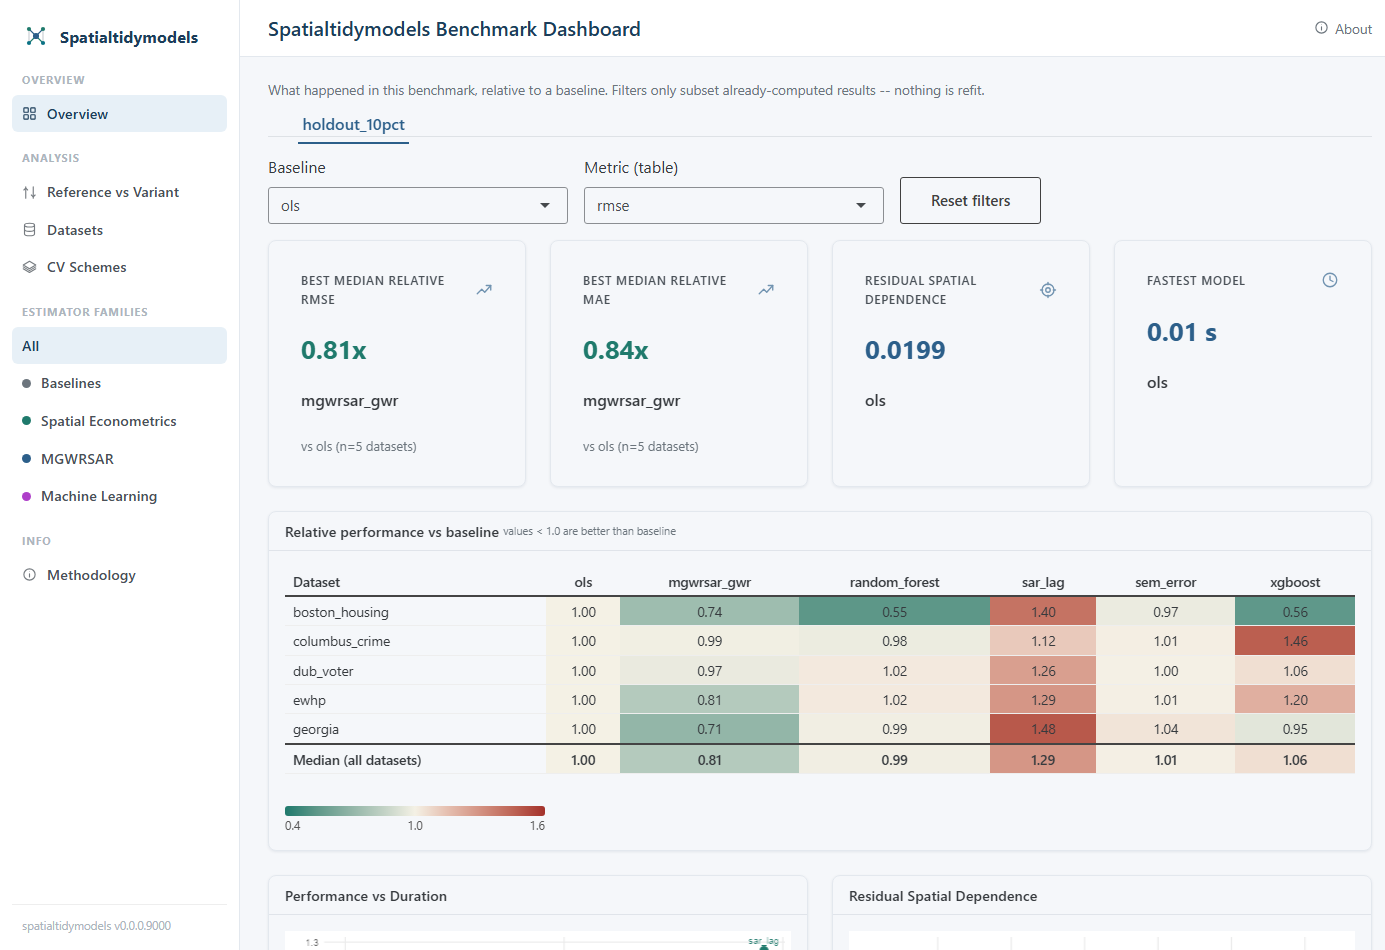
\includegraphics[width=0.90\textwidth]{dashboard_screenshot.png}
    \caption{Tableau de bord interactif de \texttt{spatialtidymodels}.}
    \label{fig:dashboard}
\end{figure}

\subsection{Difficultés rencontrées et démarche de diagnostic}

L'automatisation de la curation a fait apparaître des erreurs difficiles à repérer, car elles n'interrompent pas forcément l'exécution du pipeline. Lors de la génération des fiches de jeux de données, certaines informations peuvent ainsi être mal renseignées dans les blocs de métadonnées, notamment pour les variables, la formule ou la typologie du jeu. La présence d'une fiche complète ne suffit donc pas à garantir la validité de son contenu. J'ai dû relire manuellement certaines fiches et les confronter aux données ou à l'article source. Cette vérification a par exemple permis d'identifier, dans un jeu épidémiologique, une p-valeur du test de Mann-Kendall utilisée comme covariable en plus de la statistique dont elle était issue.

Le dédoublonnage constitue une autre difficulté importante, car un même jeu peut apparaître dans plusieurs packages, sous des noms différents ou dans des versions proches. Le pipeline applique donc plusieurs niveaux de contrôle. Il repère automatiquement certains doublons structurellement identiques et signale les cas plus ambigus lorsque les noms sont proches mais que la taille ou le nombre de variables diffèrent. Un rapprochement entre les catalogues R et Python permet également d'identifier les jeux présents dans les deux écosystèmes. Ces règles doivent rester prudentes afin d'éviter de fusionner à tort des jeux réellement distincts.

Les données de panel ont également demandé une attention particulière. Le nombre de lignes ne correspond pas au nombre d'unités spatiales distinctes, puisqu'une même unité peut apparaître à plusieurs dates. Si l'on construit directement les voisinages à partir de toutes les lignes, on obtient des coordonnées répétées et une structure spatiale potentiellement incorrecte. J'ai donc séparé l'identification des unités spatiales de la dimension temporelle avant la construction des objets utilisés par les estimateurs.

Les tests de validation croisée ont aussi révélé des problèmes qui n'auraient pas été visibles en ajustement interne. Un estimateur pouvait fonctionner sur les données d'entraînement tout en produisant des prédictions inutilisables sur un pli de test, ce qui a conduit à mieux séparer les étapes d'ajustement, de prédiction et de calcul des métriques. Un autre problème est apparu lors d'un benchmark sur \texttt{lasrosas}, un jeu de données agricoles portant sur le rendement du maïs en Argentine en fonction notamment des apports d'azote. Avec plus de 3\,000 observations, son exécution a révélé un problème de passage à l'échelle : le calcul restait bloqué sans produire de message d'erreur. J'ai isolé successivement les étapes d'ajustement, de prédiction et de diagnostic afin d'identifier l'étape responsable. Le ralentissement provenait du calcul du critère d'information d'Akaike pour un modèle de boosting, qui nécessite ici une estimation coûteuse des degrés de liberté effectifs. J'ai remplacé ce calcul par une expression déjà disponible dans l'objet estimé, puis ajouté un délai maximal d'exécution afin qu'un cas pathologique ne bloque pas l'ensemble du benchmark.


\subsection{État actuel et apports de la mission}

Le projet a produit deux composantes complémentaires : un catalogue documenté de jeux de données et une infrastructure permettant de les exploiter dans des benchmarks. Le catalogue compte actuellement 289 fiches, dont 153 issues d'articles scientifiques, 74 de packages R et 62 de packages Python. Parmi elles, 155 ont été retenues pour une intégration au package, tandis que 53 restent en révision manuelle et 81 ont été écartées du périmètre. Cette sélection ne doit pas être confondue avec l'exposition effective dans le benchmark : 117 jeux disposent actuellement d'un statut \texttt{benchmark\_ready}, et 16 exemples sont directement embarqués dans le package pour garantir un fonctionnement autonome minimal.

\begin{table}[h]
\centering
\small
\begin{tabular}{lrr}
\toprule
& Effectif & Part \\
\midrule
\multicolumn{3}{l}{\textit{Par origine}} \\
Articles scientifiques & 153 & 53\,\% \\
Packages R & 74 & 26\,\% \\
Packages Python & 62 & 21\,\% \\
\midrule
\multicolumn{3}{l}{\textit{Par statut de sélection}} \\
Retenus pour intégration au package & 155 & 54\,\% \\
En révision manuelle & 53 & 18\,\% \\
Écartés du périmètre & 81 & 28\,\% \\
\midrule
\multicolumn{3}{l}{\textit{Par état opérationnel}} \\
Benchmark-ready & 117 & 40\,\% \\
Exemples embarqués dans le package & 16 & 6\,\% \\
\midrule
\multicolumn{3}{l}{\textit{Par structure spatiale}} \\
Coupe transversale (spatial pur) & 237 & 82\,\% \\
Panel spatio-temporel & 52 & 18\,\% \\
\midrule
\multicolumn{3}{l}{\textit{Licence, parmi les jeux retenus}} \\
Licence identifiée et tracée à la source & 152 & 98\,\% \\
Source non identifiable & 3 & 2\,\% \\
\bottomrule
\end{tabular}
\caption{Composition du catalogue de jeux de données.}
\label{tab:composition-catalogue}
\end{table}

La sélection d'un jeu ne signifie pas qu'il a déjà traversé l'ensemble du moteur de benchmark. Elle indique que les données et les informations nécessaires à son exploitation ont été suffisamment documentées. Le statut \texttt{benchmark\_ready} correspond à un niveau plus exigeant : formule exécutable, variable réponse, covariables, géométrie ou coordonnées, et bloc d'éligibilité des estimateurs cohérents. La campagne de benchmark à grande échelle reste donc distincte du travail de constitution et de préparation de la banque.

Le tableau~\ref{tab:jeux-diversite} illustre la diversité des jeux retenus. Les exemples couvrent plusieurs domaines et disposent d'une spécification empirique reliée à une publication scientifique.

\begin{table}[htbp]
\centering
\footnotesize
\begin{tabularx}{\textwidth}{@{}p{2.6cm}p{2.0cm}rXrp{2.6cm}p{1.8cm}@{}}
\toprule
Jeu de données & Domaine & N & Réponse Y & X & Source (DOI) & Estimateurs éligibles \\
\midrule
Boston housing & Immobilier & 506 & valeur médiane du logement, continue & 13 & \url{https://doi.org/10.1016/0095-0696(78)90006-2} & référence non spatiale et modèles spatiaux \\
COVID sociodemographic risk & Santé publique & 3\,068 & mortalité COVID-19, continue & 15 & \url{https://doi.org/10.5061/dryad.4j0zpc8j1} & 11 variantes \\
Dragonfly diversity Europe & Macroécologie & 4\,192 & richesse spécifique, comptage & 3 & \url{https://doi.org/10.5061/dryad.78j8g} & 11 variantes \\
Florida crash GSVCM & Transport & 11\,249 & nombre d'accidents, comptage & 6 & \url{https://doi.org/10.6084/m9.figshare.12156975} & 11 variantes \\
Seshat social complexity & Histoire quantitative & 307 & population de la polity, continue & 3 & \url{https://doi.org/10.17916/p6159w} & 11 variantes \\
Airbnb Europe prices & Économie urbaine & 51\,707 & prix logarithmé, continue & 12 & \url{https://doi.org/10.5281/zenodo.4446043} & 11 variantes \\
\bottomrule
\end{tabularx}
\vspace{0.15cm}

\raggedright\scriptsize Note : la colonne « Estimateurs éligibles » indique le nombre ou la famille de routes que les métadonnées autorisent à tester ; elle ne constitue pas encore un résultat de performance.
\caption{Exemples de jeux de données issus de domaines différents.}
\label{tab:jeux-diversite}
\end{table}

Le développement de \texttt{spatialtidymodels} a permis de relier ce catalogue à une infrastructure commune d'estimation, de validation et de comparaison. Les tests réalisés au cours du développement ont également permis d'identifier plusieurs erreurs dans l'orchestration des benchmarks, notamment sur la prédiction hors échantillon, la récupération des paramètres spatiaux et le calcul des métriques après concaténation des prédictions.

Ma contribution a principalement porté sur la structuration du système de métadonnées, le développement et l'amélioration des pipelines de collecte et de curation, l'organisation du corpus autour du wiki et du graphe de connaissances, ainsi que le développement de \texttt{spatialtidymodels} et de ses outils de benchmark.


\subsection{Utilité du dispositif pour l'INRAE et la communauté scientifique}

La banque de données et \texttt{spatialtidymodels} réduisent le travail nécessaire pour évaluer une nouvelle méthode. Sans infrastructure commune, chaque comparaison demande de rechercher des jeux adaptés, de retrouver leur spécification, de préparer les données et de construire un protocole de validation. Le système développé rassemble désormais une partie de ces étapes dans un cadre commun et réutilisable.

L'intérêt du projet dépasse toutefois son usage interne à l'unité. Le package et la banque ont vocation à être mis à disposition des chercheurs afin qu'ils puissent tester de nouveaux estimateurs sur des jeux documentés et selon des schémas d'évaluation communs. Leur diffusion, notamment à terme à travers CRAN pour le package, doit faciliter la reproductibilité des comparaisons et permettre à d'autres équipes de réutiliser ou d'étendre le dispositif.

La préparation d'un \textit{data paper} complète cette démarche en documentant la banque, ses sources et les choix de curation. À ce stade, l'infrastructure est en place, mais la campagne de benchmark à grande échelle reste à conduire avant de pouvoir tirer des conclusions générales sur les performances relatives des estimateurs.

\subsection{Limites actuelles et perspectives}

La collecte produit beaucoup de jeux candidats, mais seule une partie d'entre eux passe l'ensemble des étapes de sélection. Certains sont trop peu documentés, ne peuvent pas être reliés clairement à une publication ou ne remplissent pas les critères retenus pour la banque. Les pipelines doivent donc être relancés sur de nouvelles sources tout en conservant des filtres stricts sur la présence d'une variable réponse, de covariables, d'une structure spatiale et d'une source méthodologique vérifiable.

La publication de \texttt{spatialtidymodels} sur CRAN constitue une perspective, mais elle suppose encore de stabiliser la distribution des données, la documentation des dépendances et les contrôles de conformité du package. L'architecture retenue distingue déjà les jeux embarqués, utiles pour les exemples reproductibles immédiats, et la banque complète, appelée à être hébergée dans un dépôt public consultable depuis le package. Cette organisation permettrait de maintenir l'outil léger tout en donnant accès à l'ensemble de la ressource.

Le projet se poursuivra également avec la rédaction d'un \textit{data paper}, dont le plan a commencé à être préparé. L'article présentera la banque, son système de métadonnées, les méthodes de collecte et de curation ainsi que son articulation avec \texttt{spatialtidymodels}. La rédaction devra s'appuyer sur une version gelée du catalogue et du code afin de disposer d'une référence stable et reproductible. L'objectif sera de documenter la ressource et sa construction, et non de classer les estimateurs selon leurs performances.

Une étude bibliométrique viendra compléter ce travail. Elle examinera la place accordée aux données réelles dans les articles qui développent de nouvelles méthodes spatiales, en comparant notamment le nombre de configurations étudiées par simulation avec le nombre de jeux empiriques mobilisés. Le protocole est déjà défini, mais l'étude reste à réaliser. Le corpus actuel servira de pilote avant la constitution d'un échantillon plus adapté à cette analyse.

% ============================ CONCLUSION ============================
\section{Conclusion}

La problématique de départ portait sur la rareté d'un matériel de test standardisé et diversifié pour valider des méthodes spatiales et spatio-temporelles. Le stage a permis de transformer cette difficulté en une infrastructure concrète : un catalogue documenté de jeux de données, un graphe de connaissances reliant publications, sources et spécifications, et un package R capable d'exécuter des benchmarks selon des schémas d'évaluation comparables.

L'apport principal n'est donc pas seulement quantitatif. Il ne s'agit pas d'avoir accumulé des fichiers, mais d'avoir défini les conditions dans lesquelles un jeu peut devenir utilisable : provenance, variable réponse, covariables, formule ou spécification empirique, support spatial, licence et statut de préparation. Cette exigence explique que tous les candidats collectés ne soient pas promus. Elle rend aussi la banque plus utile, car les absences et les limites sont documentées au lieu d'être masquées.

Le second apport concerne l'exécution. \texttt{spatialtidymodels} fournit une interface commune pour des estimateurs hétérogènes, un registre de méthodes, des schémas d'évaluation adaptés aux données spatiales, un moteur de comparaison appariée et un tableau de bord qui restitue les verdicts sans les recalculer. Les tests réalisés ont surtout servi à stabiliser cette infrastructure et à détecter des problèmes concrets de prédiction, de métriques ou de temps de calcul. Ils ne permettent pas encore de conclure de manière générale sur la supériorité d'un estimateur.

Ce travail ouvre donc une suite claire : gel d'une version du catalogue, consolidation des jeux \texttt{benchmark\_ready}, exécution d'une campagne de benchmark plus large, puis rédaction d'un \textit{data paper}. Il ouvre aussi une perspective méthodologique plus large pour l'unité : disposer d'un support commun pour tester de nouveaux estimateurs sur des données réelles, en complément des preuves théoriques et des simulations de Monte-Carlo.

Le cursus de Master a constitué un appui direct, notamment à travers les enseignements en économétrie, en programmation et en intelligence artificielle. Le stage m'a également permis d'approfondir mes connaissances en économétrie spatiale et d'explorer des dimensions moins présentes dans ma formation initiale, comme l'utilisation des graphes de connaissances, des outils agentiques et le développement d'un package R.

Au-delà des outils développés, je retiens surtout l'importance du diagnostic et de la vérification. Les problèmes rencontrés au cours du stage ont souvent nécessité de revenir aux données, aux sources ou au code avant de pouvoir les corriger. L'utilisation des modèles de langage a renforcé cette exigence : ils permettent de traiter un volume d'information difficilement accessible manuellement, mais leur apport reste conditionné à la possibilité de vérifier les résultats qu'ils produisent.

% ============================ ANNEXES ============================
\clearpage
\appendix

\section{Annexe 1 : Synthèse technique du pipeline}
\label{annexe:pipeline}

Cette annexe résume les éléments techniques qui sous-tendent le rapport. Elle ne remplace pas la documentation du dépôt, mais donne une vue d'ensemble du chemin suivi par un jeu candidat avant son utilisation dans \texttt{spatialtidymodels}.

\subsection{Trois pipelines de collecte}

Le projet combine trois voies de collecte. Elles ne produisent pas directement les mêmes objets, mais convergent vers les mêmes couches de curation : fiches wiki, objets spatiaux \texttt{sf}, graphe de connaissances et registre du package.

\begin{figure}[H]
\centering
\resizebox{\textwidth}{!}{%
\begin{tikzpicture}[
  node distance=0.75cm and 0.8cm,
  every node/.style={font=\scriptsize, align=center},
  source/.style={draw=myblue!70, fill=blue!6, rounded corners, text width=4.2cm, minimum height=1.05cm},
  pipeStep/.style={draw=mygray!70, fill=black!3, rounded corners, text width=4.2cm, minimum height=1.05cm},
  output/.style={draw=mygreen!75, fill=mygreen!8, rounded corners, text width=4.2cm, minimum height=1.05cm},
  final/.style={draw=myred!75, fill=myred!8, rounded corners, text width=5.4cm, minimum height=1.05cm},
  arr/.style={-{Latex[length=2mm]}, thick, mygray}
]
\node[source] (src) {Sources de jeux de données};

\node[source, below left=1.0cm and 5.2cm of src] (datacite) {Pipeline DataCite\\métadonnées de dépôts indexés};
\node[source, below=1.0cm of src] (papers) {Pipeline articles scientifiques\\DataCite, revues, Dryad ou Zenodo};
\node[source, below right=1.0cm and 5.2cm of src] (packages) {Pipeline packages\\R et Python};

\node[pipeStep, below=0.65cm of datacite] (datacite2) {Filtrage, dédoublonnage, enrichissement\\Crossref et OpenAlex};
\node[pipeStep, below=0.65cm of papers] (papers2) {PDF, données brutes, BibTeX\\et conversion GROBID};
\node[pipeStep, below=0.65cm of packages] (packages2) {Extraction et inspection locale\\des objets distribués};

\node[pipeStep, below=0.65cm of papers2] (kg) {Curation et preuves\\dans le graphe de connaissances};
\node[pipeStep, below=0.65cm of packages2] (pkgdoc) {Documentation et audit\\des sources};

\node[output, below=1.25cm of kg, xshift=-2.5cm] (wiki) {Fiches wiki de jeux\\et contrôle qualité};
\node[output, below=1.25cm of kg, xshift=2.5cm] (sf) {Objets spatiaux \texttt{sf}\\et métadonnées normalisées};

\node[final, below=0.85cm of kg, yshift=-3.0cm] (registry) {Registre \texttt{spatialtidymodels}\\\texttt{package\_include}: \texttt{yes}, \texttt{manual\_review}, \texttt{no}};
\node[final, below=0.7cm of registry] (bench) {Benchmark reproductible\\des estimateurs spatiaux};

\draw[arr] (src) -- (datacite);
\draw[arr] (src) -- (papers);
\draw[arr] (src) -- (packages);
\draw[arr] (datacite) -- (datacite2);
\draw[arr] (papers) -- (papers2);
\draw[arr] (packages) -- (packages2);
\draw[arr] (datacite2) |- (kg);
\draw[arr] (papers2) -- (kg);
\draw[arr] (packages2) -- (pkgdoc);
\draw[arr] (pkgdoc) |- (kg);
\draw[arr] (kg) -- (wiki);
\draw[arr] (kg) -- (sf);
\draw[arr] (wiki) -- (registry);
\draw[arr] (sf) -- (registry);
\draw[arr] (registry) -- (bench);
\end{tikzpicture}}
\caption{Convergence des trois pipelines de collecte vers le registre de benchmark.}
\end{figure}

Le pipeline DataCite est un mécanisme de découverte et de préqualification : il exploite les métadonnées des dépôts, filtre les candidats et les enrichit, mais ne rend pas automatiquement un jeu utilisable. Le pipeline des articles scientifiques reprend ces candidats, ou ceux issus d'une recherche par revue, puis vérifie les preuves dans le PDF et les données. Le pipeline packages part d'objets déjà distribués dans des bibliothèques R ou Python et les documente à partir de leur inspection locale et de leurs sources.

\subsection{Chemin d'un jeu de données issu d'un papier}

\begin{center}
\small
\begin{tabularx}{\textwidth}{>{\bfseries}p{3.2cm}X}
\toprule
Étape & Rôle dans le projet \\
\midrule
Collecte & Recherche de candidats via DataCite, Dryad, Zenodo ou revues spécialisées. \\
Récupération & Téléchargement légal du PDF et des fichiers de données lorsque ceux-ci sont disponibles. \\
Bibliographie & Création ou correction de l'entrée BibTeX, avec DOI, auteurs, titre et lien vers le PDF local. \\
GROBID & Conversion du PDF en TEI pour accéder aux sections, tableaux, références et mentions de données. \\
KG & Création des relations entre papier, jeu de données, formule, variables, source et statut de curation. \\
Loader R & Transformation des fichiers bruts en objet \texttt{sf} reproductible. \\
Fiche Markdown & Documentation homogène du jeu, de sa provenance, des variables et des estimateurs éligibles. \\
Vérification & Contrôle croisé entre papier, TEI, données locales et fiche ; aucune formule n'est promue sans preuve. \\
Package & Export vers les métadonnées de \texttt{spatialtidymodels} si le statut \texttt{benchmark\_ready} est atteint. \\
\bottomrule
\end{tabularx}
\end{center}

\subsection{Rôle du graphe de connaissances}

Le graphe de connaissances sert de couche intermédiaire entre les sources brutes et les fiches finales. Il ne remplace pas le papier ou les données, mais conserve les relations utiles au raisonnement : quel papier mentionne quel jeu, quelle formule est associée à quelle réponse, quelles covariables sont documentées, quelle source a permis de récupérer les fichiers et quel statut de préparation a été attribué. Cette organisation évite de relire entièrement le corpus à chaque étape et rend les décisions de curation plus traçables.

\begin{figure}[H]
\centering
\resizebox{0.97\textwidth}{!}{%
\begin{tikzpicture}[
  node distance=0.8cm and 1.0cm,
  every node/.style={font=\scriptsize, align=center},
  dataset/.style={draw=mygreen!80, fill=mygreen!10, rounded corners, minimum width=3.2cm, minimum height=0.85cm, font=\scriptsize\bfseries},
  paper/.style={draw=myblue!70, fill=blue!7, rounded corners, text width=3.0cm, minimum height=0.9cm},
  package/.style={draw=violet!70, fill=violet!7, rounded corners, text width=2.9cm, minimum height=0.85cm},
  formula/.style={draw=myred!75, fill=myred!7, rounded corners, text width=4.8cm, minimum height=0.85cm},
  varnode/.style={draw=mygray!65, fill=black!3, rounded corners, text width=2.7cm, minimum height=0.75cm},
  decision/.style={draw=orange!80!black, fill=orange!9, rounded corners, text width=3.5cm, minimum height=0.85cm},
  edge/.style={-{Latex[length=1.8mm]}, thick, mygray}
]
\node[dataset] (lsl) {\texttt{spDataLarge::lsl}};
\node[package, left=2.0cm of lsl] (pkg) {package R\\\texttt{spDataLarge}};
\node[paper, above left=1.0cm and 0.7cm of lsl] (article) {Muenchow, Brenning\\et Richter (2012)};
\node[paper, above right=1.0cm and 0.7cm of lsl] (book) {\emph{Geocomputation with R}\\chapitre spatial-cv};
\node[varnode, right=2.0cm of lsl] (sf) {objet \texttt{sf}\\350 points\\EPSG:32717};
\node[formula, below=1.0cm of lsl] (form) {\texttt{lslpts} $\sim$ \texttt{slope + cplan + cprof}\\\texttt{+ elev + log10\_carea}};
\node[varnode, below left=0.8cm and 1.0cm of form] (y) {\texttt{lslpts}\\réponse binaire};
\node[varnode, below=0.8cm of form] (x) {\texttt{slope}, \texttt{cplan}, \texttt{cprof},\\\texttt{elev}, \texttt{log10\_carea}};
\node[varnode, below right=0.8cm and 1.0cm of form] (coord) {\texttt{x}, \texttt{y}\\coordonnées exclues de X};
\node[decision, below=1.1cm of x] (ready) {\texttt{package\_include: no}\\réponse non continue\\pour le benchmark actuel};

\draw[edge] (pkg) -- node[above]{fournit} (lsl);
\draw[edge] (article) -- node[left]{documente} (lsl);
\draw[edge] (book) -- node[right]{réutilise} (lsl);
\draw[edge] (lsl) -- node[above]{matérialisé par} (sf);
\draw[edge,myred] (lsl) -- node[right]{formule retenue} (form);
\draw[edge] (form) -- (y);
\draw[edge] (form) -- (x);
\draw[edge] (form) -- (coord);
\draw[edge] (y) -- (ready);
\draw[edge] (x) -- (ready);
\end{tikzpicture}}
\caption{Sous-graphe simplifié centré sur le jeu \texttt{spDataLarge::lsl}.}
\label{fig:kg-lsl}
\end{figure}

L'exemple LSL montre pourquoi le graphe ne sert pas seulement à accumuler des liens. Le jeu est bien documenté : il provient de \texttt{spDataLarge}, contient 350 observations ponctuelles dans le sud de l'Équateur, cinq covariables topographiques et une formule reliée à la publication de Muenchow, Brenning et Richter (2012). En revanche, la variable \texttt{lslpts} indique une présence ou absence de glissement de terrain. Le KG conserve donc simultanément la preuve d'existence du jeu, la formule exploitable et la raison de non-promotion dans le benchmark de régression continue actuel.

\subsection{Structure attendue d'une fiche de jeu}

Une fiche utilisable pour le benchmark doit contenir au minimum : la provenance du jeu, le DOI du papier ou de la source lorsqu'il existe, la variable réponse, les covariables retenues, la formule publiée ou reconstruite, le support spatial, les informations de licence, le statut de préparation et le bloc d'éligibilité des estimateurs. Les champs manquants ne doivent pas être complétés par hypothèse ; ils restent documentés comme limites ou motifs de révision.

\subsection{Exemple de fiche complète}

Le jeu \texttt{paper\_airbnb\_europe\_prices} illustre le niveau attendu pour promouvoir un jeu vers le registre du package. Il provient de l'article de Gyodi et Nawaro (2021) sur les déterminants spatiaux des prix Airbnb en Europe et des fichiers déposés sur Zenodo. La fiche associe la source bibliographique, le dépôt de données, la formule empirique, les variables disponibles localement et les estimateurs éligibles.

\begin{center}
\small
\begin{tabularx}{\textwidth}{>{\bfseries}p{3.8cm}X}
\toprule
Élément contrôlé & Contenu retenu dans la fiche \\
\midrule
Source & Article \emph{Determinants of Airbnb prices in European cities: A spatial econometrics approach}, DOI \texttt{10.1016/j.tourman.2021.104319}. \\
Données & Dépôt Zenodo \texttt{10.5281/zenodo.4446043}, 51\,707 annonces Airbnb, 10 villes européennes, coordonnées \texttt{lng}/\texttt{lat}. \\
Réponse & \texttt{log\_price}, logarithme du prix, variable continue utilisée dans le papier. \\
Covariables & Type de logement, capacité, statut de l'hôte, professionnalisation, notes, chambres, distance au centre, distance au métro, attractivité touristique et restaurants. \\
Formule système & \texttt{log\_price} $\sim$ \texttt{room\_type + person\_capacity + host\_is\_superhost + multi + biz + cleanliness\_rating + guest\_satisfaction\_overall + bedrooms + dist + metro\_dist + attr\_index + rest\_index}. \\
Support spatial & Points en WGS84, matrice de voisinage reconstruite par le benchmark selon le schéma d'évaluation. \\
Statut & \texttt{benchmark\_status: ready}, \texttt{package\_include: yes}. \\
Estimateurs éligibles & Références globales, modèles SAR/SEM/SDM, GWR et méthodes prédictives non linéaires documentées comme routes de benchmark. \\
\bottomrule
\end{tabularx}
\end{center}

Cet exemple montre la différence entre une fiche simplement descriptive et une fiche utilisable : les champs ne se limitent pas à l'existence d'un fichier spatial, mais relient explicitement le jeu, l'article, la formule, les variables réellement présentes et la décision d'éligibilité.

\subsection{Estimateurs actuellement recensés}

Le registre du package contient 28 estimateurs ou variantes, regroupés de la manière suivante.

\begin{center}
\scriptsize
\begin{tabularx}{\textwidth}{>{\bfseries}p{3.2cm}X}
\toprule
Famille & Estimateurs ou variantes \\
\midrule
Références globales & \texttt{ols}, \texttt{earth}, \texttt{earth\_xy}, \texttt{gam\_spatial} \\
SAR, SEM, SDM & \texttt{sar\_lag}, \texttt{sem\_error}, \texttt{sdm\_mixed} \\
GWR et MGWRSAR & \texttt{mgwrsar\_gwr}, \texttt{mgwrsar\_mgwr}, \texttt{mgwrsar\_sar}, \texttt{mgwrsar\_mgwrsar}, \texttt{MGWRSAR\_0\_kc\_kv}, \texttt{MGWRSAR\_1\_kc\_kv} \\
Boosting & \texttt{gamboost}, \texttt{spboost}, \texttt{spboost\_bspa\_sar\_ml}, \texttt{spboost\_bspa\_sar\_cfe}, \texttt{spboost\_bspa\_sem\_ml}, \texttt{spboost\_bspa\_sem\_cfe} \\
Forêts et gradient boosting & \texttt{random\_forest}, \texttt{random\_forest\_xy}, \texttt{xgboost}, \texttt{xgboost\_xy}, \texttt{spatialml\_grf}, \texttt{spatialrf}, \texttt{rfgls} \\
Filtres spatiaux & \texttt{spmoran\_esf}, \texttt{spmoran\_resf} \\
\bottomrule
\end{tabularx}
\end{center}

Tous ne répondent pas à la même logique statistique. Certains estiment un paramètre spatial explicite, d'autres exploitent l'information géographique par les covariables, et d'autres servent de références non spatiales. Cette distinction est conservée dans les résultats du benchmark.

\begin{center}
\scriptsize
\begin{tabularx}{\textwidth}{>{\bfseries}p{2.7cm}p{4.0cm}X}
\toprule
Famille conceptuelle & Écriture schématique & Rôle dans le benchmark \\
\midrule
Régression globale & $y = X\beta + \varepsilon$ & Référence non spatiale, utile pour mesurer le gain éventuel des modèles spatiaux. \\
SAR lag & $y = \rho Wy + X\beta + \varepsilon$ & Modélise une dépendance directe de la réponse entre unités voisines. \\
SEM error & $y = X\beta + u,\quad u=\lambda Wu+\varepsilon$ & Modélise l'autocorrélation dans le terme d'erreur. \\
SDM & $y = \rho Wy + X\beta + WX\theta + \varepsilon$ & Combine dépendance sur la réponse et effets des covariables voisines. \\
GWR / MGWR & $y_i = X_i\beta(s_i)+\varepsilon_i$ & Autorise des coefficients variables dans l'espace ; MGWR permet plusieurs échelles spatiales. \\
Forêts, boosting et MARS & $y = f(X,\mathrm{coords})+\varepsilon$ & Références prédictives non linéaires ; l'information spatiale peut entrer par coordonnées ou variables dérivées. \\
Filtres spatiaux & $y = X\beta + E\gamma + \varepsilon$ & Ajoutent des composantes spatiales, par exemple des vecteurs propres de Moran. \\
\bottomrule
\end{tabularx}
\end{center}

La taxonomie doit encore être stabilisée dans les métadonnées du package. La convention utile est de distinguer trois niveaux : la famille statistique générique, le moteur logiciel utilisé et la route concrète du benchmark. Par exemple, un estimateur peut appartenir à la famille SAR, être ajusté par le package \texttt{spboost}, et apparaître dans le tableau de bord sous une route explicite comme \texttt{spboost\_bspa\_sar\_ml}. Cette séparation évite de mélanger méthode, package et variante d'implémentation.

\subsection{Outils utiles aux assistants IA}

Le dépôt contient aussi des outils destinés à rendre le travail des assistants plus contrôlable. Les serveurs MCP locaux donnent accès à des fonctions spécialisées sans relire tout le dépôt : recherche dans le catalogue de jeux, mémoire de code, compression de sorties terminal, gestion du contexte et requêtes compactes. Les compétences de Matt Pocock installées localement servent plutôt à structurer le travail d'ingénierie : revue de code, diagnostic de bogues, modélisation de domaine, conception de modules, rédaction pédagogique, développement piloté par les tests et transformation d'un plan en tâches.

\begin{center}
\small
\begin{tabularx}{\textwidth}{>{\bfseries}p{3.5cm}X}
\toprule
Famille d'outils & Usage dans le projet \\
\midrule
MCP \texttt{dataset\_search} & Interroger rapidement le catalogue de jeux et éviter de relire les fiches une par une. \\
MCP \texttt{codebase\_memory} & Repérer les fichiers, fonctions, imports et dépendances utiles dans le code. \\
MCP \texttt{context\_store}, \texttt{rtk}, \texttt{headroom} & Résumer de longues sorties terminal ou de grands blocs de contexte avant raisonnement. \\
Compétences de revue et diagnostic & \texttt{code-review}, \texttt{diagnosing-bugs}, \texttt{tdd} pour contrôler les modifications et stabiliser les scripts. \\
Compétences de conception & \texttt{domain-modeling}, \texttt{codebase-design}, \texttt{teach}, \texttt{to-prd}, \texttt{to-issues} pour formaliser le vocabulaire, les décisions et les tâches. \\
\bottomrule
\end{tabularx}
\end{center}


\clearpage


% ============================ REFERENCES ============================
\section*{Références}

{\small
\RaggedRight
\setlength{\parindent}{0pt}
\setlength{\parskip}{0.12cm}

\textbf{Méthodes spatiales et spatio-temporelles}\\[0.15cm]

Anselin, L. (1988). \textit{Spatial Econometrics: Methods and Models}. Dordrecht: Springer. \url{https://doi.org/10.1007/978-94-015-7799-1}\\[0.2cm]

Bivand, R., Millo, G. \& Piras, G. (2021). A review of software for spatial econometrics in R. \textit{Mathematics}, 9(11), 1276. \url{https://doi.org/10.3390/math9111276}\\[0.2cm]

Brunsdon, C., Fotheringham, A. S. \& Charlton, M. E. (1996). Geographically weighted regression: a method for exploring spatial nonstationarity. \textit{Geographical Analysis}, 28(4), 281--298. \url{https://doi.org/10.1111/j.1538-4632.1996.tb00936.x}\\[0.2cm]

Cliff, A. D. \& Ord, J. K. (1973). \textit{Spatial Autocorrelation}. London: Pion.\\[0.2cm]

Fotheringham, A. S., Yang, W. \& Kang, W. (2017). Multiscale geographically weighted regression (MGWR). \textit{Annals of the American Association of Geographers}, 107(6), 1247--1265. \url{https://doi.org/10.1080/24694452.2017.1352480}\\[0.2cm]

Geniaux, G. \& Martinetti, D. (2018). A new method for dealing simultaneously with spatial autocorrelation and spatial heterogeneity in regression models. \textit{Regional Science and Urban Economics}, 72, 74--85. \url{https://doi.org/10.1016/j.regsciurbeco.2017.04.001}\\[0.2cm]

Geniaux, G. (2026). Top-down scale approaches for multiscale GWR with locally adaptive bandwidths. \textit{Journal of Geographical Systems}, 28, 27--76. \url{https://doi.org/10.1007/s10109-025-00481-4}\\[0.2cm]

Lee, L.-F. (2004). Asymptotic distributions of quasi-maximum likelihood estimators for spatial autoregressive models. \textit{Econometrica}, 72(6), 1899--1925. \url{https://doi.org/10.1111/j.1468-0262.2004.00558.x}\\[0.2cm]

Legendre, P. (1993). Spatial autocorrelation: trouble or new paradigm? \textit{Ecology}, 74(6), 1659--1673. \url{https://doi.org/10.2307/1939924}\\[0.2cm]

Murakami, D. \& Griffith, D. A. (2019). Spatially varying coefficient modeling for large datasets: eliminating N from spatial regressions. \textit{Spatial Statistics}, 30, 39--64. \url{https://doi.org/10.1016/j.spasta.2019.02.003}\\[0.4cm]

\textbf{Estimateurs statistiques et apprentissage automatique}\\[0.15cm]

Breiman, L. (2001). Random forests. \textit{Machine Learning}, 45, 5--32. \url{https://doi.org/10.1023/A:1010933404324}\\[0.2cm]

Bühlmann, P. \& Hothorn, T. (2007). Boosting algorithms: regularization, prediction and model fitting. \textit{Statistical Science}, 22(4), 477--505. \url{https://doi.org/10.1214/07-STS242}\\[0.2cm]

Chen, T. \& Guestrin, C. (2016). XGBoost: a scalable tree boosting system. In \textit{Proceedings of the 22nd ACM SIGKDD International Conference on Knowledge Discovery and Data Mining}, 785--794. \url{https://doi.org/10.1145/2939672.2939785}\\[0.2cm]

Friedman, J. H. (1991). Multivariate adaptive regression splines. \textit{The Annals of Statistics}, 19(1), 1--67. \url{https://doi.org/10.1214/aos/1176347963}\\[0.2cm]

Nelder, J. A. \& Wedderburn, R. W. M. (1972). Generalized linear models. \textit{Journal of the Royal Statistical Society: Series A}, 135(3), 370--384. \url{https://doi.org/10.2307/2344614}\\[0.4cm]

\textbf{Évaluation, comparaison de méthodes et validation croisée spatiale}\\[0.15cm]

Demšar, J. (2006). Statistical comparisons of classifiers over multiple data sets. \textit{Journal of Machine Learning Research}, 7, 1--30. \url{https://www.jmlr.org/papers/v7/demsar06a.html}\\[0.2cm]

Olson, R. S., La Cava, W., Orzechowski, P., Urbanowicz, R. J. \& Moore, J. H. (2017). PMLB: a large benchmark suite for machine learning evaluation and comparison. \textit{BioData Mining}, 10, 36. \url{https://doi.org/10.1186/s13040-017-0154-4}\\[0.2cm]

Roberts, D. R., Bahn, V., Ciuti, S., Boyce, M. S., Elith, J., Guillera-Arroita, G. \textit{et al.} (2017). Cross-validation strategies for data with temporal, spatial, hierarchical, or phylogenetic structure. \textit{Ecography}, 40(8), 913--929. \url{https://doi.org/10.1111/ecog.02881}\\[0.2cm]

Schratz, P., Muenchow, J., Iturritxa, E., Richter, J. \& Brenning, A. (2019). Hyperparameter tuning and performance assessment of statistical and machine-learning algorithms using spatial data. \textit{Ecological Modelling}, 406, 109--120. \url{https://doi.org/10.1016/j.ecolmodel.2019.06.002}\\[0.2cm]

Thiyagalingam, J., Shankar, M., Fox, G. \& Hey, T. (2022). Scientific machine learning benchmarks. \textit{Nature Reviews Physics}, 4, 413--420. \url{https://doi.org/10.1038/s42254-022-00441-7}\\[0.2cm]

Weber, L. M., Saelens, W., Cannoodt, R., Soneson, C., Hapfelmeier, A. \textit{et al.} (2019). Essential guidelines for computational method benchmarking. \textit{Genome Biology}, 20, 125. \url{https://doi.org/10.1186/s13059-019-1738-8}\\[0.4cm]

\textbf{Données ouvertes, provenance et reproductibilité}\\[0.15cm]

Brunsdon, C. \& Comber, A. (2021). Opening practice: supporting reproducibility and critical spatial data science. \textit{Journal of Geographical Systems}, 23, 477--496. \url{https://doi.org/10.1007/s10109-020-00334-2}\\[0.2cm]

Konkol, M., Kray, C. \& Pfeiffer, M. (2019). Computational reproducibility in geoscientific papers: insights from a series of studies with geoscientists and a reproduction study. \textit{International Journal of Geographical Information Science}, 33(2), 408--429. \url{https://doi.org/10.1080/13658816.2018.1508687}\\[0.2cm]

Sandve, G. K., Nekrutenko, A., Taylor, J. \& Hovig, E. (2013). Ten simple rules for reproducible computational research. \textit{PLoS Computational Biology}, 9(10), e1003285. \url{https://doi.org/10.1371/journal.pcbi.1003285}\\[0.2cm]

Wilkinson, M. D., Dumontier, M., Aalbersberg, I. J., Appleton, G., Axton, M. \textit{et al.} (2016). The FAIR guiding principles for scientific data management and stewardship. \textit{Scientific Data}, 3, 160018. \url{https://doi.org/10.1038/sdata.2016.18}\\[0.4cm]

\textbf{Graphes de connaissances et modèles de langage}\\[0.15cm]

Hogan, A., Blomqvist, E., Cochez, M., d'Amato, C., de Melo, G. \textit{et al.} (2021). Knowledge graphs. \textit{ACM Computing Surveys}, 54(4), 1--37. \url{https://doi.org/10.1145/3447772}\\[0.2cm]

Liu, N. F., Lin, K., Hewitt, J., Paranjape, A., Bevilacqua, M. \textit{et al.} (2024). Lost in the middle: how language models use long contexts. \textit{Transactions of the Association for Computational Linguistics}, 12, 157--173. \url{https://doi.org/10.1162/tacl_a_00638}\\[0.2cm]

Zheng, L., Chiang, W.-L., Sheng, Y., Zhuang, S., Wu, Z. \textit{et al.} (2023). Judging LLM-as-a-judge with MT-Bench and Chatbot Arena. \textit{Advances in Neural Information Processing Systems 36} (Datasets and Benchmarks Track).\\[0.4cm]

\textbf{Outils, spécifications et littérature technique}\\[0.15cm]

GROBID (2008--2026). \textit{GROBID: GeneRation Of BIbliographic Data}. Logiciel libre. \url{https://github.com/kermitt2/grobid}\\[0.2cm]

Karpathy, A. (2026). \textit{LLM Wiki}. GitHub Gist. \url{https://gist.github.com/karpathy/442a6bf555914893e9891c11519de94f}\\[0.2cm]

Model Context Protocol (2026). \textit{Specification}. Documentation officielle. \url{https://modelcontextprotocol.io}\\[0.2cm]

}

\end{document}
